\section{Proposta}
\label{sec:proposta}

\subsection{A aplicação Price Search}

A aplicação Price Search foi pensado com o intuito de facilitar a pesquisa de preço de qualquer tipo de item existente no mercado, sejam eles eletrodomésticos, alimentos, utensílios, remédios, etc. Hoje em dia podemos encontrar diversos tipos de produtos em sites de grandes lojas, porém como existem várias cidades no Brasil que não possuem dessas grandes lojas, percebe-se que há uma grande dificuldade para saber em qual lugar tem tal item mais barato. Com isso, a ideia da aplicação é que as pessoas tenham acesso à um recurso para comparação de preço dos produtos dos estabelecimentos locais, a fim de ajudar as pessoas à economizar dinheiro. 

Outra ideia da aplicação é ajudar na busca de produtos, que antes não se sabiam onde eram vendidos. Com uma simples pesquisa, o usuário pode identificar facilmente o valor desses produtos e onde encontrá-los, por meio de um mapa que fornecerá a localização do estabelecimento contendo o seu endereço. 

O intuito é criar uma ferramenta simples, de fácil uso, e sendo ela multiplataformas, com o objetivo de agregar a quantidade máxima de usuários possíveis, para que todos possam usá-lo de maneira rápida e eficiente.

\subsection{CRUD}
No projeto haverão CRUDs (do inglês, \textit{ Create, read, update and delete}) que irão realizar as operações básicas como criar, deletar, ler ou editar as informações no banco de dados dos produtos, listas de compras, ofertas, estabelecimentos e usuários. 

\subsection{Progressive web app}

O PWA é uma aplicação \textit{web} que também se comporta como uma uma aplicação nativa e ele facilita o desenvolvimento de aplicações. Ele utiliza \textit{service workers}, que são \textit{scripts} que controlam o armazenamento de \textit{cache}, fornecendo um melhor desempenho, pois permite que os \textit{assets} e boa parte do \textit{front-end} persista armazenado no dispositivo, isso faz com que em alguns casos seja possível utiliza-lo completamente \textit{off-line}.

Mesmo sendo uma aplicação web, o PWA pode acessar grande parte dos recursos do dispositivo, como câmera, \textit{GPS} e contatos, assim podendo ser usado de forma dinâmica.

Diferente dos aplicativos que necessitam que ele seja baixado de uma loja de aplicativos, a única coisa que o usuário precisa fazer é entrar no site e caso goste ele pode salvar a aplicação \textit{web} no seu celular, como se fosse um \textit{app mobile}. E recentemente, o Google Play Store também se abriu para aplicações PWA, tornando a distribuição desse tipo de aplicação também compatível com o método convencional.


\subsection{Diagrama de Blocos}

 O diagrama de blocos é uma representação gráfica de todas as tecnologias que foram utilizadas no desenvolvimento do projeto, e de como é a comunicação entre elas.
 
\begin{figure}[!htb]
\centering
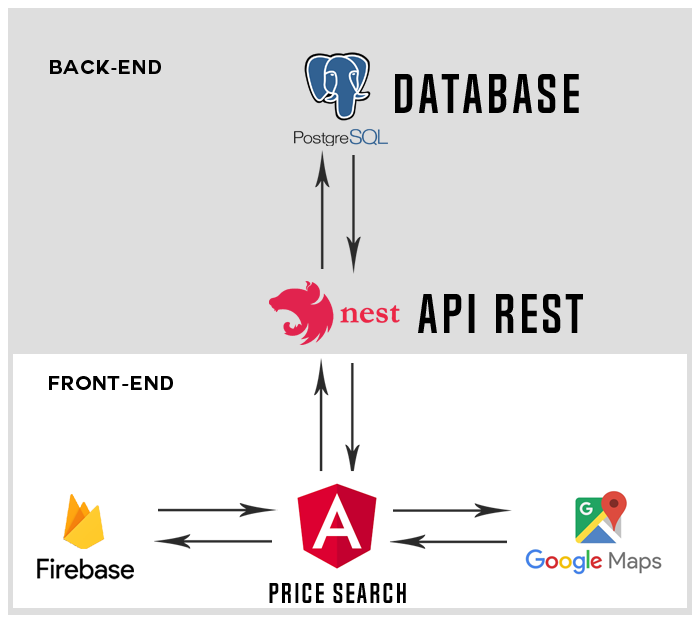
\includegraphics[width=\linewidth]{figuras/diagrama_de_blocos.png}
\caption{Diagrama de blocos da aplicação Price Search.}
\end{figure}
 
 No projeto foi utilizado PostgreSQL\footnote{Conforme explicado na seção \ref{ssec:Ambiente}} como banco de dados, NodeJs\footnote{Conforme explicado na seção \ref{ssec:NestJS}} e REST (do inglês, \textit{Representational State Transfer}\footnote{REST consiste em princípios ou regras que, quando seguidas, permitem a criação de um projeto com interfaces bem definidas. Disponível em: \url{https://becode.com.br/o-que-e-api-rest-e-restful/}}. A aplicação foi feita com Angular, e foram utilizados o Firebase para autenticação de usuário e o Google Maps Plataforma\footnote{Google Maps é um serviço de pesquisa e visualização de mapas e imagens de satélite da Terra gratuito na web. Disponível em: \url{https://www.google.com.br/}} para localização dos estabelecimentos, conforme explicado na seção \ref{sec:ferramentas}
 
\subsection{Modelo de Dados}
 
 O MER (modelo entidade relacionamento), explica como os objetos e características de um modelo de negócios se relacionam entre si. De forma geral o MER descreve como um banco de dados da aplicação é estruturado.
 
 
\begin{figure}[!htb]
\centering
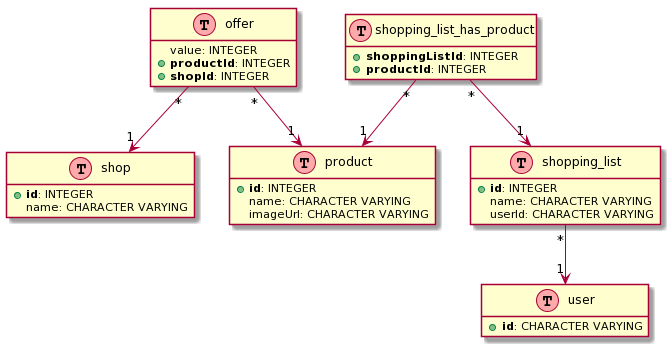
\includegraphics[width=\linewidth]{figuras/MER.png}
\caption{MER da aplicação Price Search.}
\end{figure}
 
  
 
 \subsection{Casos de Uso}
O diagrama de casos de uso da aplicação ilustra as ações de um usuário, que terá acesso às funções listadas, conforme a figura abaixo:

\begin{figure}[!htb]
\centering
\caption{Diagrama de Casos de Uso Price Search.}
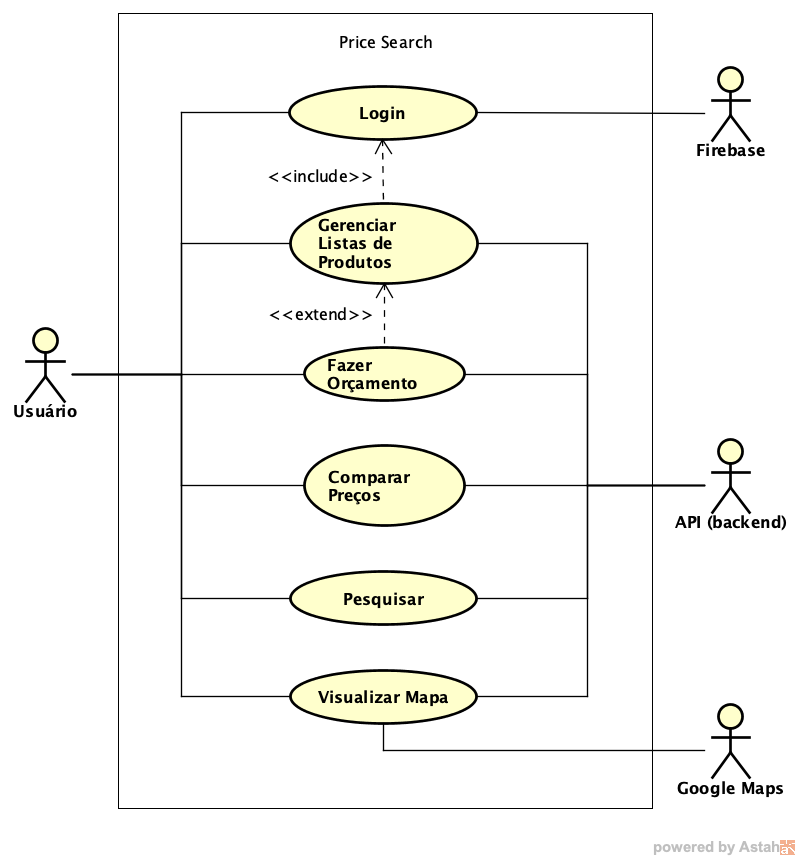
\includegraphics[width=\linewidth]{figuras/DiagramaCasosUsoPriceSearch.png}
{\footnotesize Fonte: Elaborado pelo autor.}
\end{figure}

\subsubsection{Caso de Uso 01: \textit{Login}}

O usuário inicia o login utilizando uma conta existente do Google, não sendo necessário preenchimento de nenhum tipo de dado. Feito isso, o assistente irá validar os dados do usuário e o login será efetuado. Nossa aplicação utilizará do ``token'' fornecido pela conta do Google, para que possa ser salvo em nosso banco de dados para a sincronização das informações do usuário.

\begin{figure}[!htb]
\centering
\caption{Imagem de exemplo.}
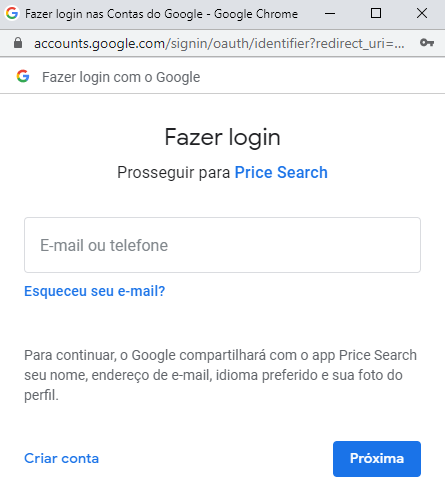
\includegraphics[width=\linewidth]{figuras/tela-login.png}
\end{figure}

\subsubsection{Caso de Uso 02: Pesquisar}

A barra de pesquisa se encontra no topo da página, junto dela também existe um botão de menu para mostrar todas as abas do aplicativo. A pesquisa será feita através do nome do produto, então o usuário poderá pesquisar por qualquer item, desde que o mesmo esteja no banco de dados, e o sistema irá retornar todos os itens de acordo com a pesquisa feita.

\begin{figure}[!htb]
\centering
\caption{Imagem de exemplo.}
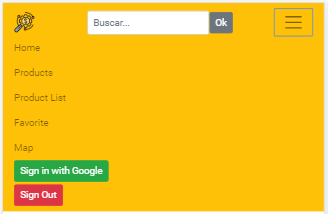
\includegraphics[width=\linewidth]{figuras/tela-menu.png}
\end{figure}

\subsubsection{Caso de Uso 03: Gerenciar Lista de Compra}

O usuário poderá criar várias listas de compra como se fosse um carrinho de compras. Ao criar uma lista, o usuário poderá escolher um nome para ela; bem como escolher quais itens serão adicionados futuramente, e removê-los a qualquer momento; ou mesmo renomear a lista ou exclui-lá.

\begin{figure}[!htb]
\centering
\caption{Tela onde mostram todos os produtos disponíveis.}
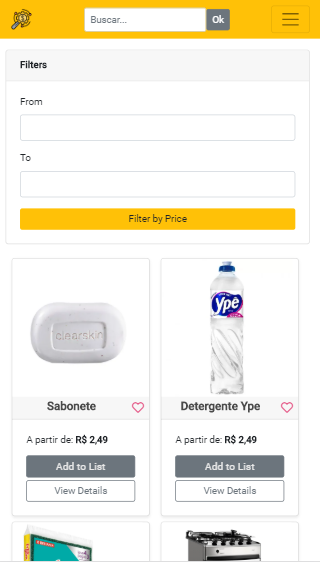
\includegraphics[width=\linewidth]{figuras/tela_lista_produtos.png}
\end{figure}

\subsubsection{Caso de Uso 04: Comparar Preços}

O usuário poderá comparar preços de um produto em diferentes estabelecimentos, e através do aplicativo descobrir em qual estabelecimento ele pode encontrar o melhor preço do produto que deseja.

\begin{figure}[!htb]
\centering
\caption{Imagem de exemplo.}
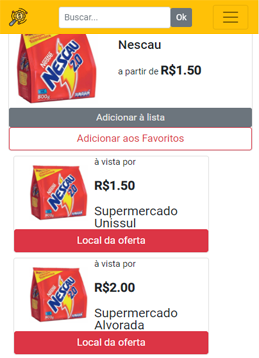
\includegraphics[width=\linewidth]{figuras/tela-comparar.png}
\end{figure}

\subsubsection{Caso de Uso 05: Fazer Orçamento}

O usuário poderá criar listas de compras, e ao fazer isso ele poderá realizar o orçamento, e descobrir em qual estabelecimento a compra ficará mais barata.

\begin{figure}[!htb]
\centering
\caption{Imagem de exemplo.}

\includegraphics[width=\linewidth]{figuras/placeholder.jpg}
\end{figure}

\subsubsection{Caso de Uso 06: Visualizar Mapa}

O usuário terá acesso à um mapa que contém a localização de todos os estabelecimentos locais cadastrados. Ao clicar nos estabelecimentos mostrados no mapa, irá ser fornecido informações sobre ele, como nome e endereço.


\begin{figure}[!htb]
\centering
\caption{Imagem de exemplo.}
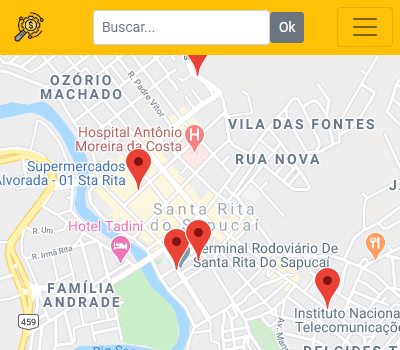
\includegraphics[width=\linewidth]{figuras/tela_mapa.png}
\end{figure}
